%%=============================================================================
%% Methodologie
%%=============================================================================

\chapter{Methodologie}
\label{ch:methodologie}

\section{De keuze van de spraakassistenten}
Omdat het gaat over een vergelijkend onderzoek, is het belangrijk in weinig veranderlijke omstandigheden te werken. Om te vermijden dat de hardware een invloed heeft op de resultaten worden de assistenten gebruikt op hetzelfde toestel, de Xiami Redmi Note 4. Hierdoor kregen bepaalde assistenten geen kans meer om opgenomen te worden in het onderzoek. Bixby is enkel beschikbaar op apparaten van Samsung zoals Siri enkel beschikbaar is voor Apple-gebruikers. Daarnaast heeft het ontwikkelen van eigen applicaties beperkingen voor beide assistenten.

--vertel hier nog over welke beperkingen precies--

Na eerder opgesomde redenen wordt beslist om enkel Amazon Alexa en Google Assistant verder te onderzoeken. Meer specifiek zal de Amerikaans-Engelse Alexa vergeleken worden met de Amerikaans-Engelse Google Assistant en de Nederlandstalige Google Assistant uit Nederland.


\section{Wat wordt er vergeleken}
\label{sec:vergelijking van stemgestuurde assistenten}
--Hier nog over de twee dingen die worden onderzocht: spraakherkenning en spraaksynthese + verwijzing naar stand van zaken--
--dan verdere onderverdeling: spraaksynthese aan de hand van de kwaliteit. 5 eigenschappen: verstaanbaarheid, menselijkheid, levendigheid, tempo en emotionaliteit en extra uitleg--
--spraakherkenning wordt er vergeleken hoe goed de assistent spraak heeft omgevormd naar tekst door het aantal fouten te meten. Hoe correct een assistent een bepaalde vraag van de gebruiker kan begrijpen door te meten hoe sterk zijn gevormde zin verschilt van de gestelde vraag--

\section{Gebruikte materialen}
Voor het onderzoek zijn volgende zaken gebruikt:
\begin{itemize}
    \item Acer Aspire F 15 laptop
    \begin{itemize}
        \item Intel Core I5
        \item geïntegreerde microfoon
        \item 2,5 jaar in gebruik
    \end{itemize}
    \item Xiami Redmi note 4 smartphone
    \begin{itemize}
        \item Android 7.0
        \item Octa core processor
        \item 4 GB RAM
        \item 2 jaar in gebruik
    \end{itemize}
    \item Ultimate Ears BOOM 2 Speaker
    \begin{itemize}
        \item 12,5 watt vermogen
        \item 90dB gevoeligheid
        \item 3,5mm mini-jack (AUX) ingang
        \item 1,5 jaar in gebruik
    \end{itemize}
    \item 3.5mm Jack kabel
    \item Google Assistant app voor Android
    \item Alexa Beta app voor Android
\end{itemize}

\section{Het verloop van het onderzoek}
\subsection{Deel één: met de deelnemer}
De steekproef bestaat uit 30 Vlamingen tussen 19 en 60 jaar die Nederlands spreken als moedertaal en enige kennis hebben van de Engelse taal. Het onderzoek is afgenomen in twee grote delen.

De onderzoeker volgt voor dit deel een vast stappenplan die te vinden is in \ref{appendix:stappenplan proefafname}.
De vragenlijst die tijdens dit deel wordt ingevuld is te vinden onder de map bijlagen in de repository beschreven in \ref{s:verwijzing naar repository}.
Er is een kleine applicatie ontwikkeld voor elke assistent waar de gebruiker EHBO-gerelateerde vragen aan kan stellen en telkens een vast antwoord van terugkrijgt.

\begin{figure}[h]
    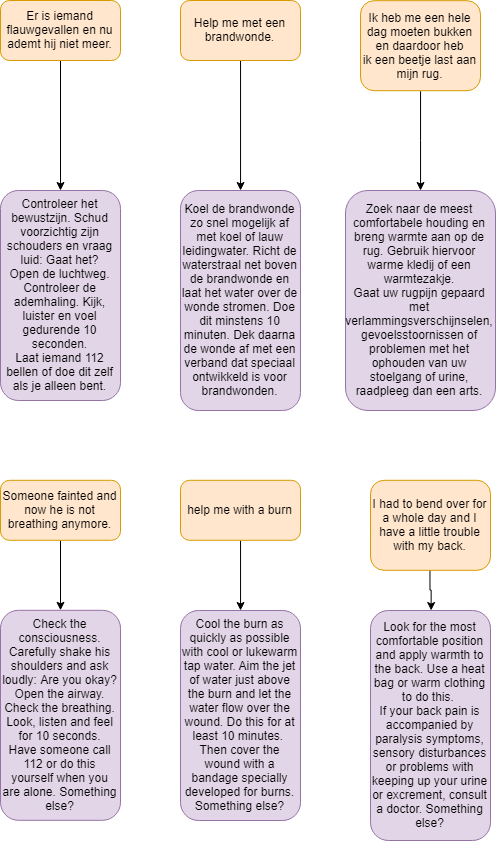
\includegraphics[width=0.7\linewidth]{img/flowdiagram_testapp}
    \caption{De flowchart waar de applicaties voor de test op zijn gebaseerd}
    \label{fig:flowdiagram}
\end{figure}

Voor het eerste deel stellen de deelnemers drie Engelse en drie Nederlandse EHBO-gerelateerde vragen aan een fictieve spraakassistent. De gestelde vragen worden opgenomen door een laptop.
Om te beginnen leest de deelnemer een korte introductietekst over spraakassistenten en vult hij enkele algemene vragen in. Daarna krijgt hij zes bladeren met op elk blad een vraag. Hij wordt aangespoord door de onderzoeker om elke vraag eerst in stilte te lezen om hem daarna te stellen aan de assistent. De aanwezigheid van een spraakassistent wordt geveinsd omdat de manier waarop de deelnemer de vragen stelt vergelijkbaar moet zijn aan de manier waarop hij ze zou stellen aan een echte assistent. De participant krijgt nooit een antwoord te horen, waardoor de mogelijkheid ontstaat dat hij steeds meer zijn best doet de volgende vraag duidelijker uit te spreken. Het verkregen resultaat zijn opgenomen audiofragmenten die later worden gebruikt in het tweede deel.

Na het stellen van alle vragen wordt de deelnemer op de hoogte gebracht van de assistent zijn afwezigheid en krijgt hij een volgende taak. Hij moet nu aan drie bestaande assistenten telkens dezelfde drie vragen stellen en te luisteren naar de drie antwoorden. Hij krijgt de antwoorden van de assistent te horen door een speaker die met een kabel is aangesloten aan een smartphone. Hij kan de vragenlijst over de assistenten hun spraakkwaliteit al eens doornemen. De participant wordt door de onderzoeker aangespoord om goed te luisteren. Hij mag vragen opnieuw stellen tot hij antwoord krijgt van de assistent. Telkens nadat een assistent de drie vragen heeft beantwoord wordt de vragenlijst over die assistent ingevuld. De deelnemer krijgt na elke beoordeling de kans om vorige beoordelingen van assistenten aan te passen. Op het einde vult de participant nog enkele algemene vragen in.

\begin{figure}[h]
    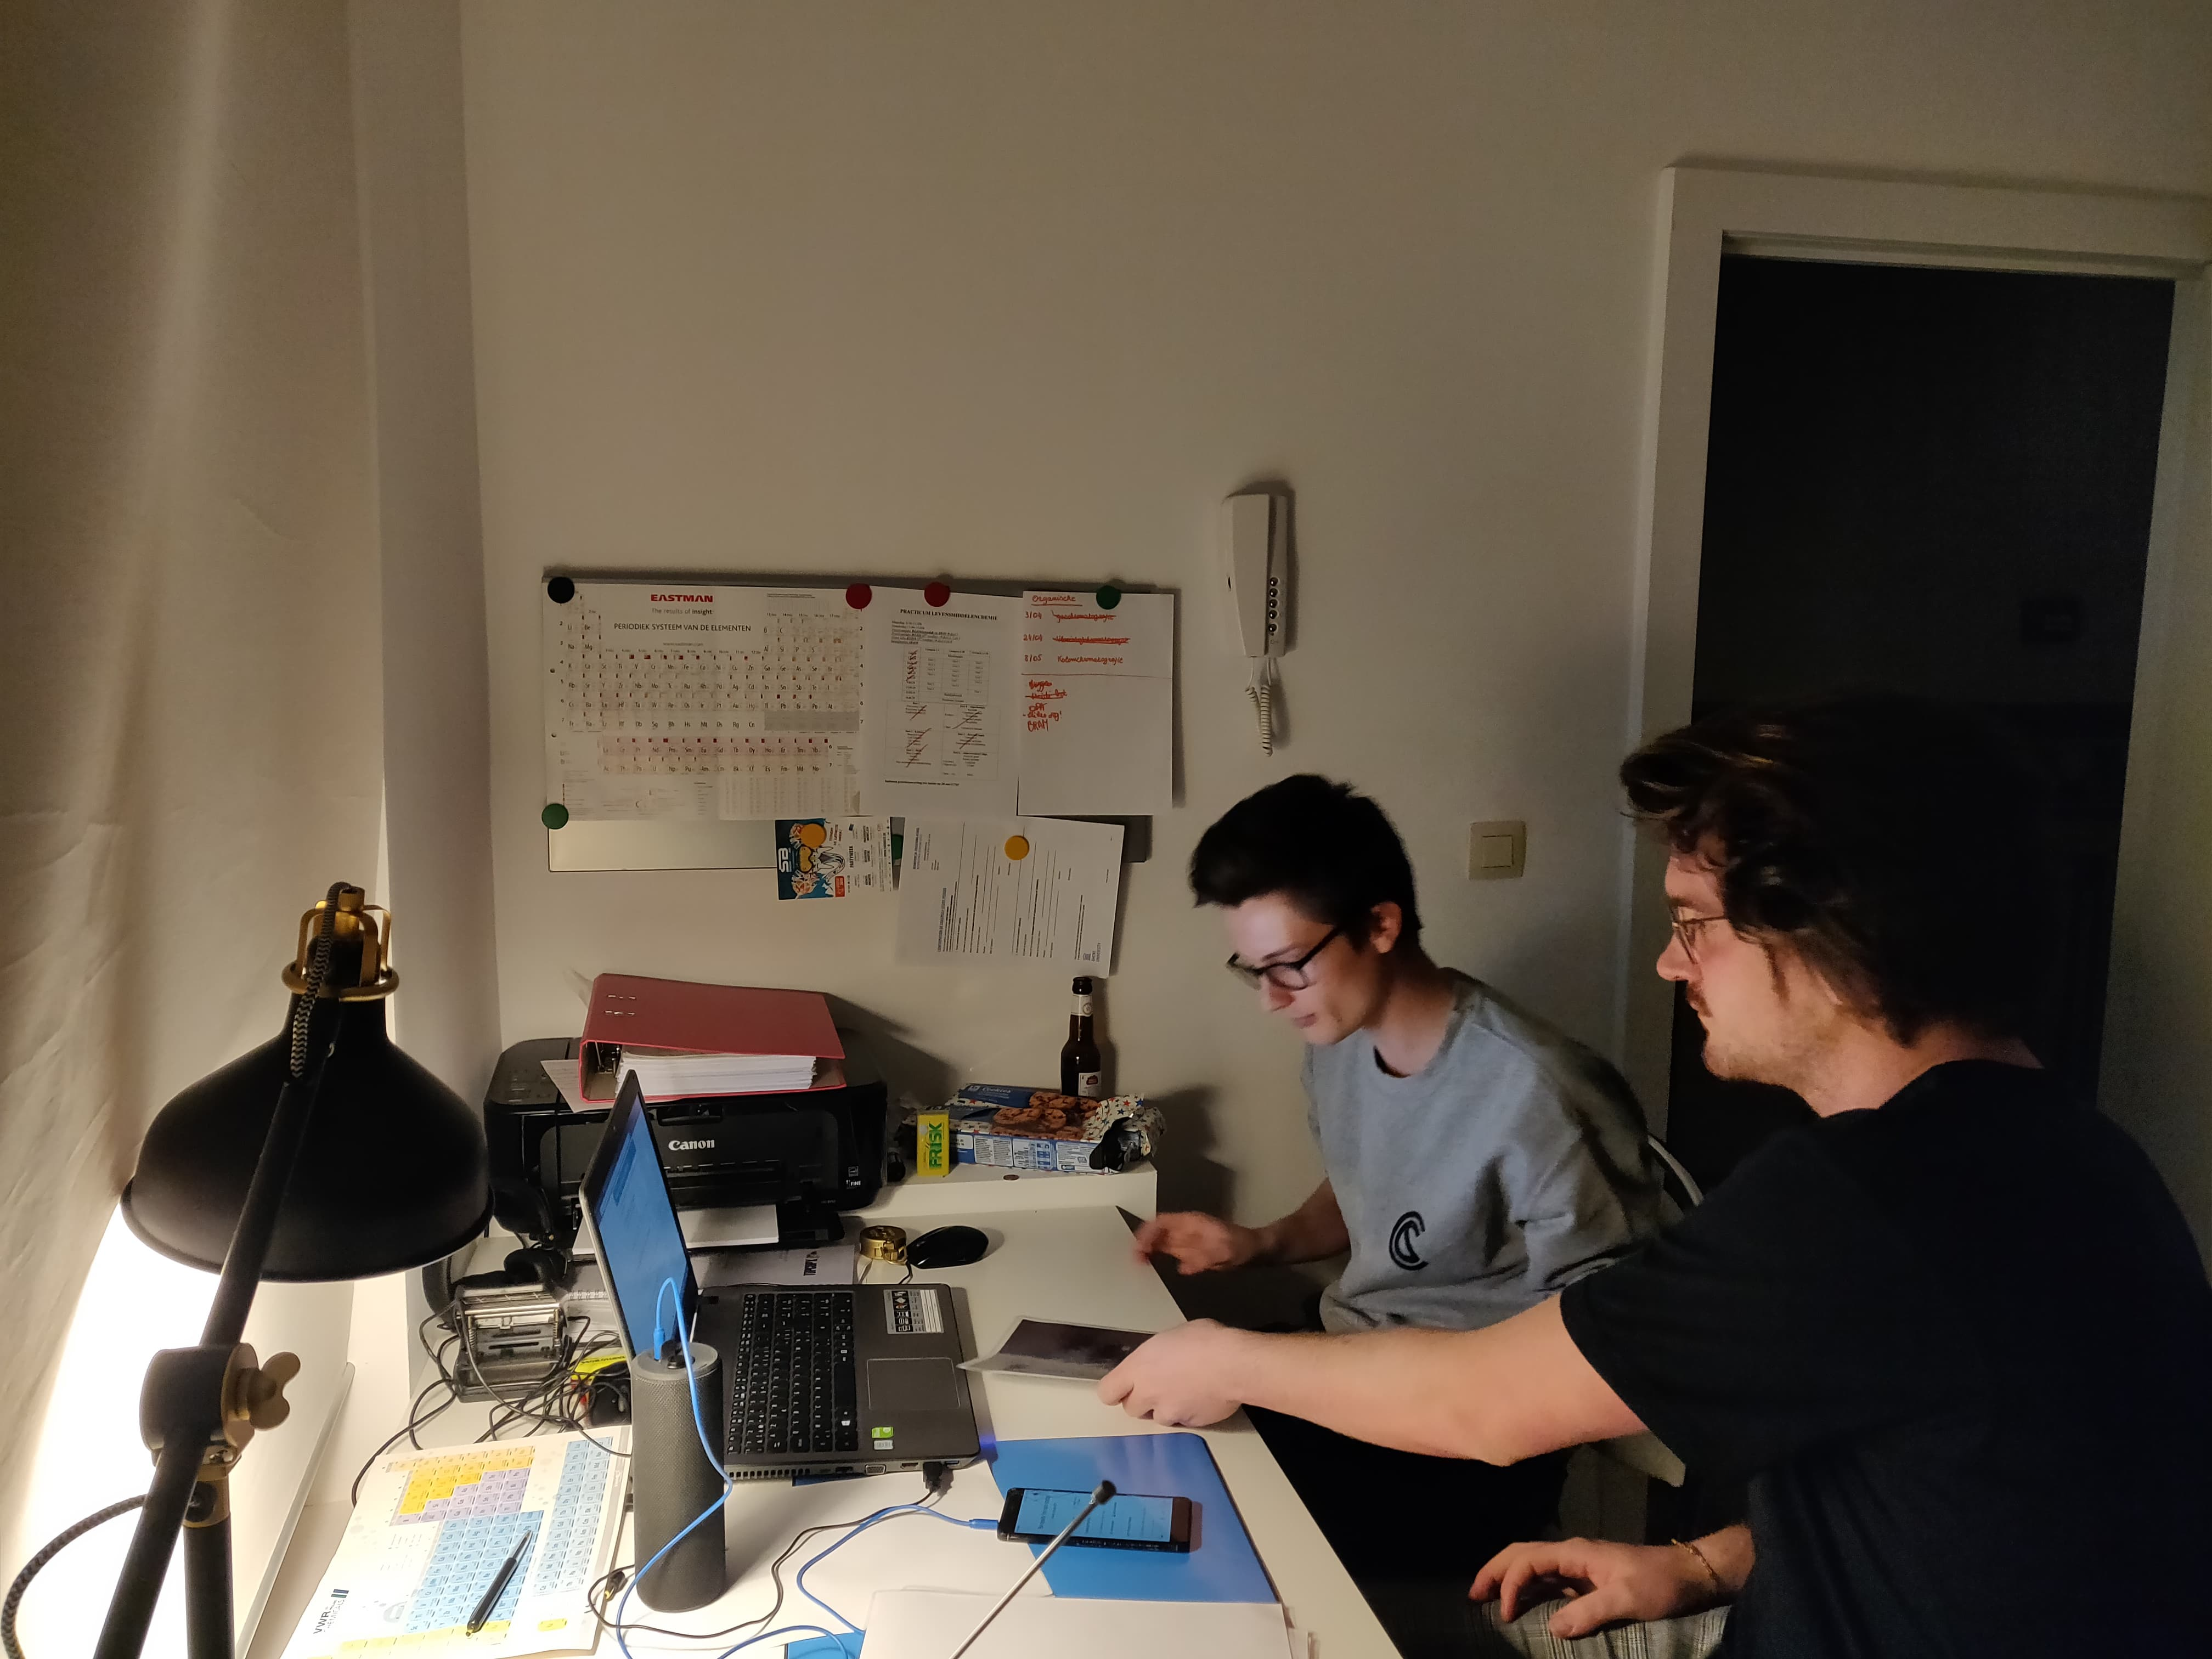
\includegraphics[width=0.7\linewidth]{img/proefafname2}
    \caption{Een deelnemer ontvangt de vragen die hij zal stellen aan de assistenten.}
    \label{fig:proefafname1}
\end{figure}

\subsection{Deel twee: zonder de deelnemer}
De vragenlijst die tijdens dit deel wordt ingevuld is te vinden onder de map bijlagen in de repository beschreven in \ref{s:verwijzing naar repository}.

Tijdens het tweede deel van het onderzoek luisteren de assistenten naar de vragen van de deelnemer. Er wordt gemeten hoe de assistenten deze vragen van spraak omzetten naar tekst.
Er werden maatregelen genomen om de beïnvloeding van veranderlijke factoren te beperken. Een persoon zal nooit twee keer een vraag op exact dezelfde manier uitspreken. Als de deelnemer elke vraag al kan stellen zonder versprekingen dan nog zal er altijd een verschil zijn in onder meer volume, snelheid en intonatie. Daarnaast is er ook nog de extra beïnvloeding van externe ruis.

Een oplossing kan zijn om drie toestellen te gebruiken die elk voorzien zijn van een andere assistent. De gebruiker kan dan de vraag eenmalig stellen terwijl de drie assistenten tegelijkertijd luisteren. Ondanks dat dit op het eerste zicht een goede oplossing lijkt, zijn er toch enkele bedenkingen. Wegens financiële redenen is het voor de onderzoeker niet mogelijk om drie nieuwe smartphones aan te kopen. Moest dit toch mogelijk zijn dan kan er nog steeds een verschil van kwaliteit in de microfoon aanwezig zijn. Elk apparaat is uniek. Als er met drie gebruikte smartphones wordt gewerkt zal het verschil zeker aanwezig zijn door slijtage of ongelijk model.

Dit is de reden waarom de vragen zijn opgenomen in deel één. Een geregistreerd audiofragment maakt het mogelijk om de identieke vraag drie keren af te spelen terwijl telkens één assistent meeluistert op hetzelfde apparaat. Dit gebeurt in een geluidsdichte opnamestudio om externe ruis tijdens dit proces zoveel mogelijk te beperken. Er kan wel ruis mee opgenomen zijn tijdens deel één, maar die is dan aanwezig bij elke assistent die het audiofragment hoort. De fragmenten worden afgespeeld door een speaker die aangesloten is op een laptop met een kabel.

\begin{figure}[h]
    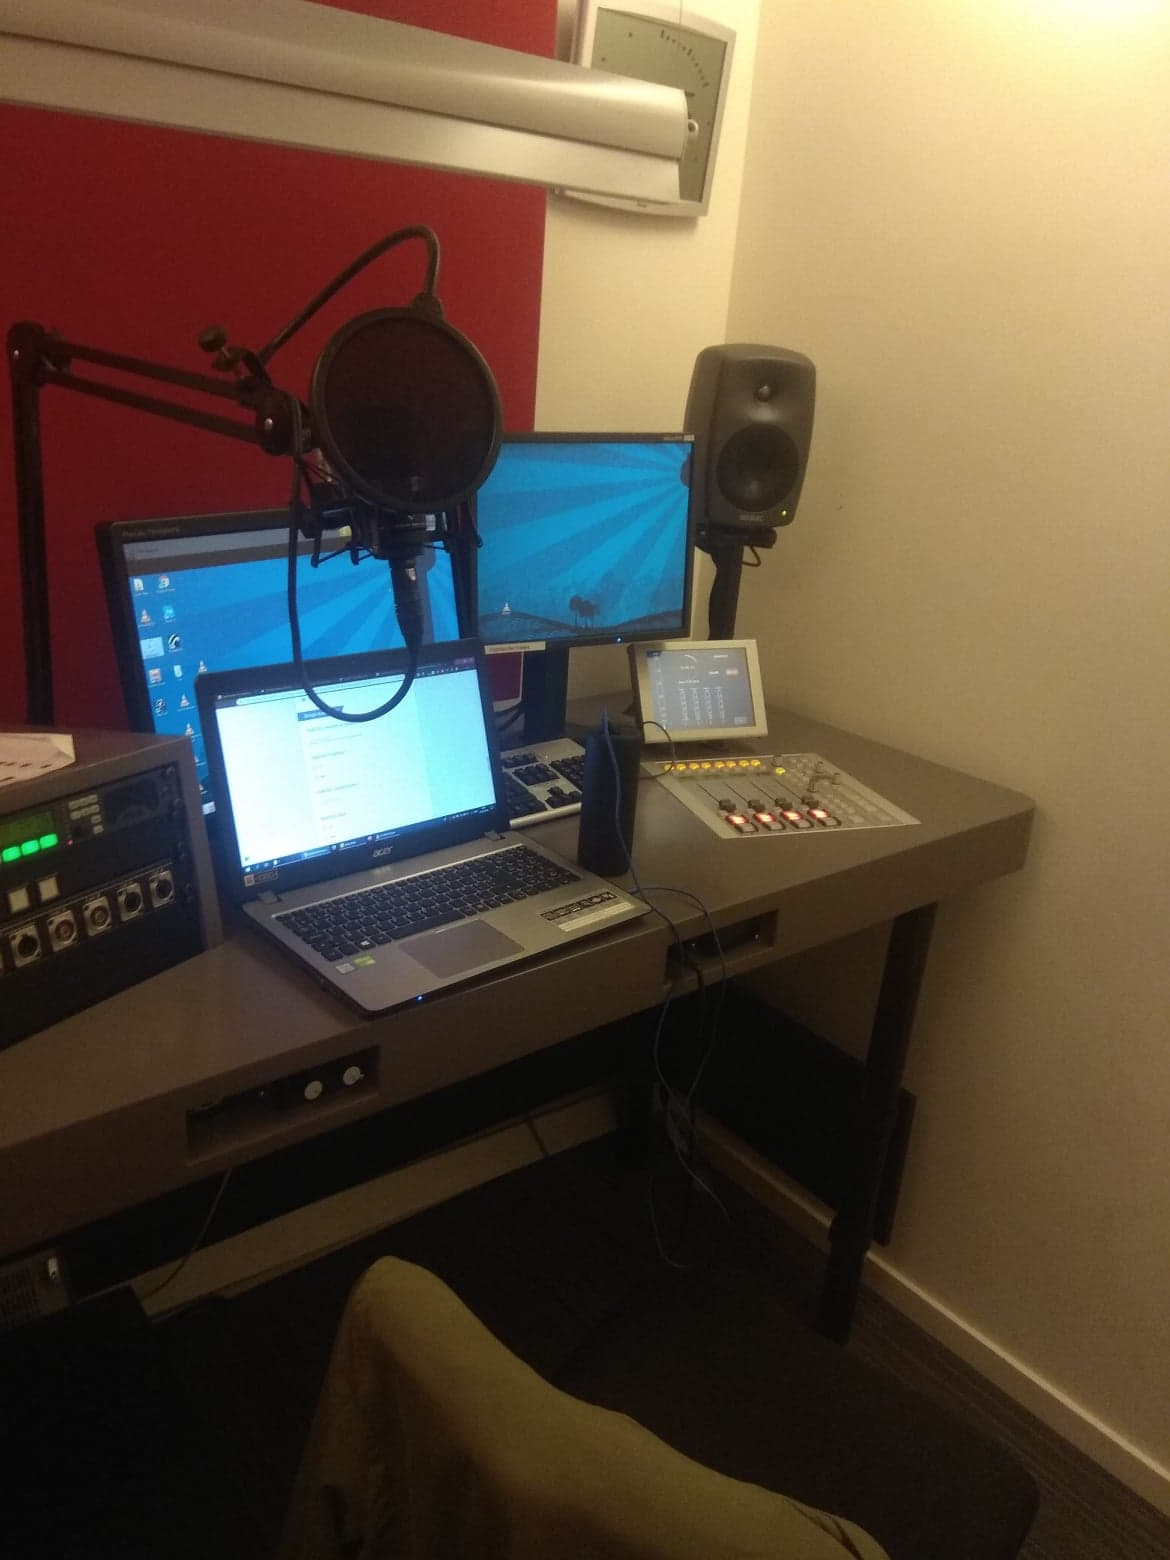
\includegraphics[width=0.7\linewidth]{img/proefafname3}
    \caption{De audiofragmenten worden beluisterd door de assistenten in een geluidsdichte studio.}
    \label{fig:proefafname2}
\end{figure}

Zowel Alexa als Google Assistant maken het mogelijk om een overzicht van uw interacties te bekijken. Na de audiofragmenten van de 30 gebruikers af te spelen voor elke assistent werd dit overzicht gebruikt om de vragenlijst in te vullen. In de vragenlijst wordt de omgezette tekst van de assistent genoteerd samen met het aantal fouten die het bevat.

\subsection{Ontwikkelen van een applicatie}
\label{sec:ontwikkelen van een applicatie}
Welke middelen kan je gebruiken om het te ontwikkelen?

Hoe uitgebreid is de documentatie?

Welke programmeertalen worden aangeboden?

Kan de applicatie automatisch een nummer bellen?

\section{Orthopedagogisch onderzoek}
\label{Orthopedagogisch onderzoek}
\subsection{De zoektocht naar een gepaste doelgroep}
\label{De zoektocht naar een gepaste doelgroep}

\subsubsection{Ondersteuning van de begeleider in de jeugdzorg}
\label{ondersteuning van de begeleider in de jeugdzorg}
De aanleiding van dit onderzoek was een onderzoek van -citeer onderzoek mr. Buysse- over faciliterende IT bij individuele begeleidingsgesprekken in de jeugdzorg. Uit het onderzoek ontstond er twijfel over het gebruik van een spraakassistent als ondersteuning bij het individuele begeleidingsgesprek tussen de persoonlijke begeleider en het kind. Door de twijfel werd er dan ook beslist om niet verder te gaan met spraaktechnologie, maar met andere digitale tools.

Om er toch zeker van te zijn dat er geen mogelijkheden waren, ontstond deze bachelorproef. Echter, na een eerste gesprek met Iris Storme, docent orthopedagogie binnen Hogeschool Gent en tevens mede-researcher van -citeer onderzoek mr. Buysse- werden voor mij de beweegredenen voor het afkeuren van spraaktechnologie binnen hun onderzoek snel duidelijk. 

Als je denkt aan mensen met een visuele of fysieke beperking komen er snel mogelijkheden naar boven. Denk maar aan het controleren van apparaten met een eenvoudig stemcommando. Deze personen kunnen technologie als een mogelijke oplossing zien, waardoor zij, en de begeleiders, dit gemakkelijker kunnen omarmen.
Daartegenover staat de bijzondere jeugdzorg, waar de spraakassistent eerder ondersteuning zou bieden in de emotionele problematiek en de jongeren net hun façade nodig hebben om overeind te blijven. Deze doelgroep stelt zich niet zo graag kwetsbaar op en ervaart het praten over gevoelens eerder als een drempel. De bijzondere jeugdzorg lijkt op het eerste zicht een minder relevante doelgroep.

Dit werd allemaal vastgesteld door het intuïtieve gevoel van de ondervraagde. Dit was voor mij persoonlijk voldoende om na te gaan denken over een nieuwe doelgroep.

\subsubsection{Ondersteuning van personen met het syndroom van Down}
\label{ondersteuning van personen met het syndroom van Down}
Ik wijzigde mijn doelgroep naar personen die geboren zijn met trisomie 21, ook wel het syndroom van Down genoemd. Uit een eerste opzoeking stelde ik de volgende mogelijkheden.

Personen met het Downsyndroom worden geboren met een verstandelijke beperking. Er kan gekeken worden naar welke noden uit die verstandelijke beperking vloeien, bijvoorbeeld moeite met rekenen, en hoe een spraakassistent hier ondersteuning kan bieden. Dit kan ook veel verder gaan als in vb. het helpen met zelfstandig wonen.

Daarnaast zijn er ook mogelijke bijkomende aandoeningen zoals een minder goed geheugen, coeliakie, slaapapneu, oogafwijkingen of een gedragsstoornis. Hier kan spraakassistentie mogelijks ook ondersteuning in bieden. Ik denk aan bijvoorbeeld interactieve activiteiten voor het stimuleren van de motoriek, het geheugen of het spraakvermogen, helpen herinneren aan belangrijke taken, helpen herinneren aan wat ze wel of niet mogen eten, stimuleren van een vast slaappatroon, enzovoort.

--Bronnen vermelden--

Dit waren nog maar losse ideeën die ontstonden uit een eerste verkenning over personen met het gendefect. Het werd duidelijk dat hier zeker mogelijkheden waren, dus was de volgende stap om hierin gaan te verdiepen door interviews af te nemen van mensen die een persoonlijke ervaring hebben met deze doelgroep.

Echter, mijn eerste aanvraag voor een interview aan iemand wiens dochter geboren is met trisomie 21 stootte direct op weerstand. Het antwoord dat ik kreeg, ging over het gevaar van veralgemenen. Het is een complexe materie omdat het gaat over een combinatie van samenkomende symptomen en kenmerken. De effecten van het gendefect kunnen in verschillende gradaties voorkomen, waardoor elke persoon die het gendefect bezit uniek moet bekeken worden.